\documentclass[11pt,oneside,a4paper,openright]{report}

\usepackage{parskip}
\usepackage[utf8]{inputenc}
% Make latex understand and use the typographic
% rules of the language used in the document.
\usepackage[english]{babel}
\usepackage{lmodern}
% Choose the font encoding
\usepackage[T1]{fontenc}
\usepackage{xcolor}
\definecolor{codegray}{rgb}{0.5,0.5,0.5}
\definecolor{codepurple}{rgb}{0.58,0,0.82}
\definecolor{backcolour}{rgb}{0.95,0.95,0.92}

\usepackage{listings}

\lstdefinestyle{javastyle}{
    backgroundcolor=\color{backcolour},   
    commentstyle=\color{codegreen},
    keywordstyle=\color{codepurple},
    numberstyle=\tiny\color{codegray},
    stringstyle=\color{codepurple},
    basicstyle=\footnotesize,
    breakatwhitespace=false,         
    breaklines=true,                 
    captionpos=b,                    
    keepspaces=true,                 
    numbers=left,                    
    numbersep=5pt,                  
    showspaces=false,                
    showstringspaces=false,
    showtabs=false,                  
    tabsize=4
}
 
\lstset{style=javastyle}
% The standard graphics inclusion package
\usepackage{graphicx}
% Set up how figure and table captions are displayed
\usepackage{caption}
\captionsetup{%
  font=footnotesize,% set font size to footnotesize
  labelfont=bf % bold label (e.g., Figure 3.2) font
}

\begin{document}
\graphicspath{./}
\section{IP Miniproject - Rasmus Christiansen - Student no. 20144790}
In this miniproject I present two algorithms for scaling an image. One uses forward mapping, and the other uses backward mapping. I have chosen to present two algorithms instead of one because they both follow the same mathematical principle and it provides a good point for discussing why you would use one over the other.

The first algorithm is as follows:


\begin{lstlisting}
output_image_height = input_image_height * Sy
output_image_width = input_image_width * Sx	
for (y = 0; y < input_image_height; ++y)
{
	for (x = 0; x < input_image_width; ++x)
	{
		output_image(y*Sy, x*Sx) = input_image(y, x)
	}
}
\end{lstlisting}


When you look at this algorithm it becomes clear why this is called forward mapping. The algorithm goes through each pixel in the input image and maps it to the most appropriate output; input -> output. The downside of this is that it leaves black spots, because the algorithm goes through the input image rather than the output. This can work in other image processing algorithms where the input and output have a 1:1 relationship, but for a scaling algorithm this is never the case. Therefore, it is better to use backward mapping, which is the second algorithm i use:
\begin{lstlisting}
output_image_height = input_image_height * Sy
output_image_width = input_image_width * Sx
for (y = 0; y < output_image_height; ++y)
{
	for (x = 0; x < output_image_width; ++x)
	{
		output_image(y, x) = input_image(1 / Sy * y, 1 / Sx * x)
	}
}
\end{lstlisting}

Contrary to the first algorithm, this one goes through each pixel in the output image, and then maps the most appropriate pixel \textit{to it}. This is why it is called backward mapping. If the forward mapping algorithm pushes data, the backward mapping pulls it instead; output <- input.

\subsection{Code overview}
\subsubsection{Entirety of code}
\begin{lstlisting}
#include "opencv2/opencv.hpp"
#include <iostream>

using namespace cv;
using namespace std;

int roundNum(float num) {

	if (num - floor(num) >= 0.5)
		num = ceil(num);
	else
		num = floor(num);

	return num;
}

//Simple scaling algorithm using forward mapping
Mat simpleScaling(Mat src, float Sx, float Sy)
{

	if (Sx <= 0 || Sy <= 0)
	{
		cout << "Negative scaling is not possible";
		return src;
	}
		
	//Create a Mat object with scaled dimensions, greyscale, completely black.
	Mat output(src.rows*Sy,src.cols*Sx, CV_8U, Scalar(0, 0, 0));

	for (int y = 0; y < src.rows; ++y)
	{
		for (int x = 0; x < src.cols; ++x)
		{
			output.at<uchar>(y*Sy, x*Sx) = src.at<uchar>(y, x);
		}
	}

	return output;
}

Mat backScaling(Mat src, float Sx, float Sy)
{
	if (Sx <= 0 || Sy <= 0)
	{
		cout << "Negative scaling is not possible";
		return src;
	}

	Mat output(src.rows*Sy, src.cols*Sx, CV_8U, Scalar(0, 0, 0));
	int tmpy, tmpx;

	for (int y = 0; y < output.rows; ++y)
	{
		for (int x = 0; x < output.cols; ++x)
		{
			tmpy = roundNum(1 / Sy*y);
			tmpx = roundNum(1 / Sx*x);

			if (tmpy >= src.rows)
				tmpy = src.rows - 1;

			if (tmpx >= src.cols)
				tmpx = src.cols - 1;

			output.at<uchar>(y, x) = src.at<uchar>(tmpy, tmpx);
		}
	}
	return output;
}

int main(int, char)
{
	Mat image = imread("input.jpg");
	cvtColor(image, image, CV_BGR2GRAY);
	
	float Sx, Sy;
	cout << "Enter horizontal scalar: "; cin >> Sx; cout << endl;
	cout << "Enter vertical scalar: "; cin >> Sy; cout << endl;

	Mat image2 = simpleScaling(image, Sx, Sy);
	Mat image3 = backScaling(image, Sx, Sy);
	imshow("IMAGE", image);
	imshow("IMAGE2", image2);
	imshow("IMAGE3", image3);
	waitKey(0);
		
	return 0;
}
\end{lstlisting}

\subsubsection{Explanation of code}
Besides the main function, the code contains two functions that each contain the different scaling algorithms, and a third functions which is a basic number rounding function. The algorithm functions take an image and two floats - the scalars - as arguments.

Both scaling functions start with this if-statement:
\begin{lstlisting}
if (Sx <= 0 || Sy <= 0)
{
	cout << "Negative scaling/scaling to 0 is not possible";
	return src;
}
\end{lstlisting}
This is simple error prevention; while it could be argued that "negative" scaling could be achieved by flipping the image on both axes, that is not a feature of this software. A scalar with the value of "0" would result in an image width or height of 0 which is also no good.

The rest of the forward mapping function is as follows:
\begin{lstlisting}
//Create a Mat object with scaled dimensions, greyscale, completely black.
Mat output(src.rows*Sy,src.cols*Sx, CV_8U, Scalar(0, 0, 0));

for (int y = 0; y < src.rows; ++y)
{
	for (int x = 0; x < src.cols; ++x)
	{
		output.at<uchar>(y*Sy, x*Sx) = src.at<uchar>(y, x);
	}
}
return output;
\end{lstlisting}
So, for each pixel in the input image, it takes the most appropriate pixel of the output image, and makes it equal to the current pixel.

From executing bits of code, I found that when a floating point number is interpreted as an integer, it is simply rounded down. I wanted something a bit more precise than that, so I created this function:
\begin{lstlisting}
int roundNum(float num) {

	if (num - floor(num) >= 0.5)
		num = ceil(num);
	else
		num = floor(num);

	return num;
}
\end{lstlisting}
It simply rounds a floating point number to it's nearest integer. I found that this resulted in pixels potentially being mapped out of bounds of the output image. So besides the rounding and the backward mapping, there is another slight change to the other function. If a pixel has a position outside the array, it is simply mapped to the outmost position within the array. Here is the code:
\begin{lstlisting}
Mat output(src.rows*Sy, src.cols*Sx, CV_8U, Scalar(0, 0, 0));
int tmpy, tmpx;

for (int y = 0; y < output.rows; ++y)
{
	for (int x = 0; x < output.cols; ++x)
	{
		tmpy = roundNum(1 / Sy*y);
		tmpx = roundNum(1 / Sx*x);
		
		if (tmpy >= src.rows)
			tmpy = src.rows - 1;

		if (tmpx >= src.cols)
			tmpx = src.cols - 1;
		output.at<uchar>(y, x) = src.at<uchar>(tmpy, tmpx);
	}
}
return output;
\end{lstlisting}
The pixel position is stored in two variables. This is leftover from debugging, as the roundNum function can be called within the output.at function. 

Finally i will show the effects of this software in action. I put in 1.2 and 0.5 as my Sx and Sy scalars, and this is the result:

\begin{center}
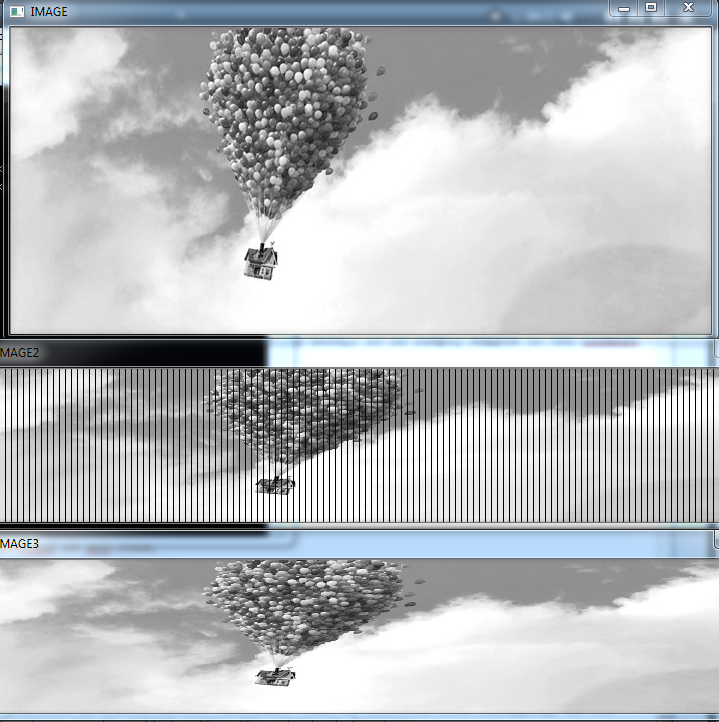
\includegraphics[scale=0.75]{result}
\end{center}
The top image is the original, the one in the middle is scaled with forward mapping and the bottom image is scaled with backward mapping. The image scaled with forward mapping has some noticeable black vertical lines which are not present on the bottom image. 

\end{document}